%=========================================================
\chapter{Modelo del Negocio}	
\label{cap:reqSist}

En este capítulo se modela la {\em Arquitectura del negocio} la cual está conformada por la Ontología del negocio (Glosario de {\em Términos}), el Modelo del Dominio del problema (entidades y relaciones), las {\em Reglas de negocio} y las {\em Máquinas de estado} que controlan el ciclo de vida de los expedientes. Primero se especifica el {\em Contexto} operativo de la organización.

%----------------------------------------------------------
\section{Contexto}

La **Fundación Futuro con Derechos** es una organización civil que se encarga de proteger y restituir de forma integral los derechos vulnerados de niñas, niños y adolescentes (NNA) en situación de orfandad por motivo de femicidio. La institución opera mediante un equipo multidisciplinario (psicólogos, médicos, trabajadores sociales y abogados) liderado por coordinadores y bajo la supervisión de la Dirección General. 

El flujo de trabajo operativo gira en torno a la detección del menor, la apertura de su expediente único, la valoración especializada en las cuatro áreas críticas, el diseño de un Plan de Restitución de Derechos (PRD) que contiene las medidas de protección específicas, y el monitoreo constante de su bienestar. El sistema web **Taimotla** tiene como finalidad digitalizar y automatizar esta estructura para evitar fugas de información, lentitud administrativa y fallos de coordinación.

%---------------------------------------------------------
\section{Términos del Negocio}
\label{sec:terminosDeNegocio}

A continuación se presenta la definición formal de los términos fundamentales de la operación de la Fundación, organizados en forma de glosario con hipervínculos cruzados:

\begin{description}
	\item[\hypertarget{tFundacion}{Fundación Futuro con Derechos:}] Organización no gubernamental dedicada a la atención integral de NNA huérfanos por femicidio en el estado de Nuevo León.
	\item[\hypertarget{tLGDNNA}{LGDNNA:}] Ley General de los Derechos de Niñas, Niños y Adolescentes. Es el marco normativo superior que rige todas las acciones y medidas de protección de la Fundación.
	\item[\hypertarget{tFUD}{FUD:}] Formulario Único de Datos. Herramienta que recopila toda la información de identidad, del hecho victimal, y del entorno social del NNA.
	\item[\hypertarget{tDirector}{Director:}] Actor del sistema. Máxima autoridad de la Fundación encargada de auditar la plataforma, gestionar las cuentas del personal y conformar los equipos.
	\item[\hypertarget{tCoordinador}{Coordinador:}] Actor del sistema. Profesional que supervisa las valoraciones y la ejecución de medidas de un equipo multidisciplinario.
	\item[\hypertarget{tAbogado}{Abogado:}] Especialista legal del equipo. Encargado de la defensa judicial y la regularización legal (tutela, custodia) del NNA.
	\item[\hypertarget{tMedico}{Médico / Doctor:}] Especialista de salud del equipo. Responsable del diagnóstico clínico, tratamiento físico y control del seguro médico del NNA.
	\item[\hypertarget{tPsicologo}{Psicólogo:}] Especialista de salud mental del equipo. Provee apoyo emocional, terapia por trauma de duelo y aplica peritajes psicológicos.
	\item[\hypertarget{tTSocial}{Trabajador Social:}] Especialista social del equipo. Realiza estudios socioeconómicos y visitas a la red familiar del menor.
	\item[\hypertarget{tEquipo}{Equipo Multidisciplinario:}] Célula de trabajo compuesta por un coordinador y especialistas que atienden un expediente específico de forma unificada.
	\item[\hypertarget{tNNA}{NNA:}] Niña, Niño o Adolescente menor de 18 años cuyos derechos han sido restringidos o vulnerados y es el beneficiario central.
	\item[\hypertarget{tTutor}{Tutor:}] Adulto que ejerce la guarda, custodia o patria potestad del NNA ante la ausencia de sus progenitores.
	\item[\hypertarget{tExpediente}{Expediente Único Digital:}] Carpeta digital en el sistema Taimotla que unifica los datos médicos, psicológicos, sociales, legales e historial del menor.
	\item[\hypertarget{tPRD}{Plan de Restitución de Derechos (PRD):}] Documento técnico-legal y de seguimiento donde se especifican las medidas de protección especial para subsanar los derechos vulnerados del menor.
	\item[\hypertarget{tMedidaUrgente}{Medida Urgente:}] Acción inmediata de resguardo físico, legal o de salud implementada ante un riesgo inminente para la vida o integridad del NNA.
\end{description}

%----------------------------------------------------------
\section{Modelo del dominio del problema}
\label{sec:hechosDeNegocio}

El modelo del dominio del problema representa gráficamente las entidades estructurales del sistema **Taimotla** y sus asociaciones. El diagrama de clases UML se detalla en la figura~\ref{fig:modeloDeDominio}.

\begin{figure}[htbp!]
	\begin{center}
		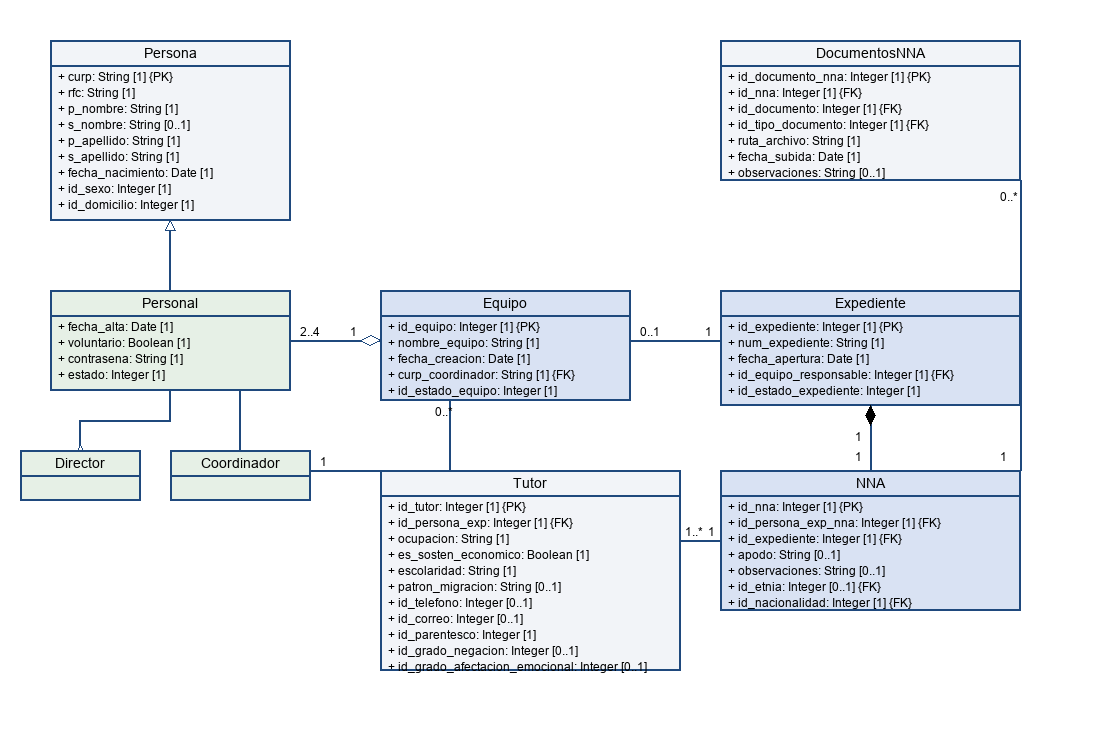
\includegraphics[width=0.95\textwidth]{images/modelo_dominio_fundacion}
		\caption{Modelo del dominio del problema para el sistema Taimotla.}
		\label{fig:modeloDeDominio}
	\end{center}
\end{figure}

A continuación se describen las entidades principales del modelo y sus relaciones:

\begin{cdtEntidad}{Persona}{Persona}
	\brAttr{curp}{CURP}{Alfanumérico (18)}{Clave Única de Registro de Población utilizada como identificador primario de toda persona en el sistema.}{Sí}
	\brAttr{rfc}{RFC}{Alfanumérico (13)}{Registro Federal de Contribuyentes.}{Sí}
	\brAttr{p\_nombre}{Primer Nombre}{Palabra Corta}{Primer nombre de la persona.}{Sí}
	\brAttr{s\_nombre}{Segundo Nombre}{Palabra Corta}{Segundo nombre, de existir.}{No}
	\brAttr{p\_apellido}{Primer Apellido}{Palabra Corta}{Primer apellido paterno.}{Sí}
	\brAttr{s\_apellido}{Segundo Apellido}{Palabra Corta}{Segundo apellido materno.}{Sí}
	\brAttr{fecha\_nacimiento}{Fecha de Nacimiento}{Fecha}{Fecha de nacimiento de la persona.}{Sí}
	\cdtEntityRelSection
	\brRel{\brRelComposition}{Domicilio}{Toda persona reside en un \hyperlink{Domicilio}{Domicilio}.}
\end{cdtEntidad}

\begin{cdtEntidad}{Personal}{Personal}
	\brAttr{fecha\_alta}{Fecha de Alta}{Fecha}{Fecha en que el empleado se incorporó a la Fundación.}{Sí}
	\brAttr{voluntario}{Voluntario}{Booleano}{Indica si el empleado es voluntario o contratado de base.}{Sí}
	\brAttr{estado}{Estado}{Entero}{Estatus de la cuenta (Habilitado/Deshabilitado).}{Sí}
	\cdtEntityRelSection
	\brRel{\brRelGeneralization}{Persona}{Un \hyperlink{Personal}{Personal} hereda todos los datos de una \hyperlink{Persona}{Persona}.}
\end{cdtEntidad}

\begin{cdtEntidad}{Equipo}{Equipo}
	\brAttr{id\_equipo}{Identificador}{Entero}{Clave autoincremental única del equipo.}{Sí}
	\brAttr{nombre\_equipo}{Nombre}{Palabra Corta}{Nombre identificador del equipo multidisciplinario.}{Sí}
	\brAttr{fecha\_creacion}{Fecha de Creación}{Fecha}{Fecha en que el Director conformó el equipo.}{Sí}
	\cdtEntityRelSection
	\brRel{\brRelComposition}{Personal}{Un \hyperlink{Equipo}{Equipo} se compone de un Coordinador y entre 2 y 4 especialistas de \hyperlink{Personal}{Personal}.}
\end{cdtEntidad}

\begin{cdtEntidad}{Expediente}{Expediente}
	\brAttr{id\_expediente}{Identificador}{Entero}{Clave única interna del expediente.}{Sí}
	\brAttr{num\_expediente}{Número de Expediente}{Alfanumérico}{Clave física y oficial asignada al caso.}{Sí}
	\brAttr{fecha\_apertura}{Fecha de Apertura}{Timestamp}{Fecha y hora en que se abrió el caso en el sistema.}{Sí}
	\brAttr{id\_estado\_expediente}{Estado}{Entero}{Identificador del estado actual del expediente.}{Sí}
	\cdtEntityRelSection
	\brRel{\brRelAgregation}{Equipo}{Un \hyperlink{Expediente}{Expediente} tiene asignado un \hyperlink{Equipo}{Equipo} para su atención.}
\end{cdtEntidad}

\begin{cdtEntidad}{NNA}{NNA}
	\brAttr{id\_nna}{Identificador}{Entero}{Clave única del menor en el sistema.}{Sí}
	\brAttr{apodo}{Apodo}{Palabra Corta}{Nombre por el cual se identifica de confianza al menor.}{No}
	\brAttr{observaciones}{Observaciones}{Texto Largo}{Notas generales del caso del menor.}{No}
	\cdtEntityRelSection
	\brRel{\brRelComposition}{Expediente}{Toda \hyperlink{NNA}{NNA} está asociada de manera exclusiva a un \hyperlink{Expediente}{Expediente}.}
	\brRel{\brRelComposition}{Tutor}{Un \hyperlink{NNA}{NNA} está vinculado a uno o varios \hyperlink{Tutor}{Tutores} o familiares directos.}
\end{cdtEntidad}

\begin{cdtEntidad}{Domicilio}{Domicilio}
	\brAttr{id\_domicilio}{Identificador}{Entero}{Clave única del domicilio en el sistema.}{Sí}
	\brAttr{calle}{Calle}{Palabra Corta}{Nombre de la calle.}{Sí}
	\brAttr{num\_ext}{Número Exterior}{Palabra Corta}{Número exterior de la vivienda.}{Sí}
	\brAttr{num\_int}{Número Interior}{Palabra Corta}{Número interior de la vivienda, de existir.}{No}
	\cdtEntityRelSection
	\brRel{\brRelComposition}{Colonia}{El domicilio pertenece a una Colonia.}
\end{cdtEntidad}

\begin{cdtEntidad}{Tutor}{Tutor}
	\brAttr{id\_tutor}{Identificador}{Entero}{Clave única del tutor en el sistema.}{Sí}
	\brAttr{ocupacion}{Ocupación}{Palabra Corta}{Ocupación u oficio del tutor.}{Sí}
	\brAttr{es\_sosten\_economico}{Sostén Económico}{Booleano}{Indica si el tutor es el principal proveedor económico.}{Sí}
	\brAttr{escolaridad}{Escolaridad}{Palabra Corta}{Último grado escolar del tutor.}{Sí}
	\brAttr{patron\_migracion}{Patrón de Migración}{Palabra Corta}{Historial o patrón de migración, de existir.}{No}
	\brAttr{observaciones}{Observaciones}{Texto Largo}{Notas adicionales sobre el tutor.}{No}
	\cdtEntityRelSection
	\brRel{\brRelGeneralization}{Persona}{Un \hyperlink{Tutor}{Tutor} hereda los datos de una \hyperlink{Persona}{Persona}.}
\end{cdtEntidad}

\begin{cdtEntidad}{HechoVictimal}{HechoVictimal}
	\brAttr{id\_hecho}{Identificador}{Entero}{Clave única del hecho victimal en el sistema.}{Sí}
	\brAttr{num\_reporte}{Número de Reporte}{Palabra Corta}{Número oficial o folio del reporte del caso.}{Sí}
	\brAttr{nombre\_caso}{Nombre del Caso}{Palabra Corta}{Nombre identificador o clave asignada al caso.}{Sí}
	\brAttr{fecha\_detencion}{Fecha de Registro}{Fecha}{Fecha en que el menor ingresó o fue puesto a disposición.}{Sí}
	\brAttr{nombre\_victima\_madre}{Víctima Madre}{Palabra Corta}{Nombre completo de la madre víctima del feminicidio.}{Sí}
	\brAttr{descripcion\_delito}{Descripción del Delito}{Texto Largo}{Detalle de los delitos relacionados en perjuicio de la familia.}{No}
	\brAttr{narracion\_sucedido}{Narración de lo Sucedido}{Texto Largo}{Narrativa sucinta de los hechos victimales.}{No}
	\cdtEntityRelSection
	\brRel{\brRelComposition}{NNA}{El hecho victimal está asociado de forma exclusiva a un \hyperlink{NNA}{NNA}.}
\end{cdtEntidad}

\begin{cdtEntidad}{Documento}{Documento}
	\brAttr{id\_documento}{Identificador}{Entero}{Clave única del documento digital en el sistema.}{Sí}
	\brAttr{nombre\_documento}{Nombre}{Palabra Corta}{Nombre oficial del documento (ej. Acta de Nacimiento).}{Sí}
	\brAttr{ruta\_archivo}{Ruta de Archivo}{Palabra Corta}{Ubicación de almacenamiento en el servidor de archivos.}{Sí}
	\brAttr{fecha\_subida}{Fecha de Subida}{Timestamp}{Fecha y hora en que se cargó el archivo digital.}{Sí}
	\brAttr{observaciones}{Observaciones}{Texto Largo}{Notas adicionales del estado o vigencia del documento.}{No}
	\cdtEntityRelSection
	\brRel{\brRelAgregation}{NNA}{El documento digital está vinculado a un \hyperlink{NNA}{NNA} en su expediente.}
\end{cdtEntidad}


%---------------------------------------------------------
\section{Modelado de Reglas de negocio}

Las reglas de negocio estructuran y restringen las operaciones lógicas de la Fundación y la base de datos. Estas se detallan a continuación:

\begin{BussinesRule}{BR-01}{Estructura obligatoria de un equipo multidisciplinario.}
	\BRitem[Tipo:] Regla de integridad estructural. 
	\BRitem[Clase:] Habilitadora. 
	\BRitem[Nivel:] Control.
	\BRitem[Descripción:] Un equipo multidisciplinario de caso debe estar compuesto de forma obligatoria por un Coordinador de Caso y un mínimo de 2 y un máximo de 4 profesionales especialistas activos (un Abogado, un Médico, un Psicólogo o un Trabajador Social).
	\BRitem[Motivación:] Garantizar el enfoque integral y la mirada interdisciplinaria exigida por el artículo 123 de la LGDNNA para la toma de decisiones.
	\BRitem[Sentencia:] $\forall e \in Equipo \Rightarrow e.coordinador \neq \emptyset \land 2 \le |e.miembros| \le 4$.
	\BRitem[Ejemplo positivo:] Un equipo integrado por un Coordinador, un Abogado y un Psicólogo cumple con la regla.
	\BRitem[Ejemplo negativo:] Un equipo sin coordinador asignado, o que contenga únicamente a un Trabajador Social como miembro, no cumple con la regla.
	\BRitem[Referenciado por:] \hyperlink{CU-02}{CU-02}, \hyperlink{CU-04}{CU-04}.
\end{BussinesRule}

\begin{BussinesRule}{BR-02}{Asignación exclusiva a equipos activos.}
	\BRitem[Tipo:] Regla de integridad estructural. 
	\BRitem[Clase:] Habilitadora. 
	\BRitem[Nivel:] Control.
	\BRitem[Descripción:] Un especialista operativo (Abogado, Médico, Psicólogo o Trabajador Social) solo puede estar asignado a un único equipo multidisciplinario activo en el sistema a la vez.
	\BRitem[Motivación:] Evitar la sobrecarga de trabajo del personal de la Fundación y asegurar la dedicación debida a los expedientes asignados.
	\BRitem[Sentencia:] $\forall p \in Personal \land e_1, e_2 \in EquiposActivos \Rightarrow p \in e_1 \Rightarrow p \notin e_2$.
	\BRitem[Ejemplo positivo:] El Abogado Juan Pérez está asignado al Equipo Alfa y no pertenece a ningún otro equipo.
	\BRitem[Ejemplo negativo:] Intentar agregar al Médico Carlos Gómez al Equipo Beta cuando ya se encuentra registrado y activo en el Equipo Alfa.
	\BRitem[Referenciado por:] \hyperlink{CU-04}{CU-04}.
\end{BussinesRule}

\begin{BussinesRule}{BR-03}{Registro de NNA con CURP obligatoria.}
	\BRitem[Tipo:] Regla de integridad referencial. 
	\BRitem[Clase:] Habilitadora. 
	\BRitem[Nivel:] Control.
	\BRitem[Descripción:] El registro de cualquier Niña, Niño o Adolescente (NNA) en el sistema requiere la captura obligatoria de una Clave Única de Registro de Población (CURP) de 18 caracteres alfanuméricos válidos y que no esté duplicada en la base de datos.
	\BRitem[Motivación:] Evitar el registro duplicado de menores y asegurar su correcta identificación jurídica.
	\BRitem[Sentencia:] $\forall n \in NNA \Rightarrow |n.CURP| = 18 \land (n_1.CURP = n_2.CURP \Rightarrow n_1 = n_2)$.
	\BRitem[Ejemplo positivo:] Registro del menor con CURP válida de 18 dígitos.
	\BRitem[Ejemplo negativo:] Intentar guardar un expediente dejando el campo CURP vacío, o ingresar una CURP que ya está registrada para otro menor en el sistema.
	\BRitem[Referenciado por:] \hyperlink{CU-03}{CU-03}.
\end{BussinesRule}

\begin{BussinesRule}{BR-04}{Carga obligatoria de documentos de identidad.}
	\BRitem[Tipo:] Regla de operación. 
	\BRitem[Clase:] Habilitadora. 
	\BRitem[Nivel:] Control.
	\BRitem[Descripción:] Un expediente de NNA no puede avanzar del estatus ``Creado'' a ``En Diagnóstico'' si el Abogado asignado no ha cargado al sistema la copia digitalizada del acta de nacimiento o el documento de identidad oficial equivalente.
	\BRitem[Motivación:] Asegurar la existencia de soporte legal de identidad antes de proceder con el diseño del Plan de Restitución.
	\BRitem[Sentencia:] $\forall ex \in Expediente \land ex.estado = \mbox{'En Diagnóstico'} \Rightarrow \exists doc \in ex.documentos \land doc.tipo = \mbox{'Acta de Nacimiento'}$.
	\BRitem[Ejemplo positivo:] El Abogado sube el acta de nacimiento en PDF y el sistema permite iniciar el registro de valoraciones.
	\BRitem[Ejemplo negativo:] El equipo intenta registrar diagnósticos médicos o psicológicos sin haber cargado el acta de nacimiento previa.
	\BRitem[Referenciado por:] \hyperlink{CU-03}{CU-03}.
\end{BussinesRule}

\begin{BussinesRule}{BR-05}{Pre-autorización y aprobación del Plan de Restitución (PRD).}
	\BRitem[Tipo:] Regla de inferencia. 
	\BRitem[Clase:] Habilitadora. 
	\BRitem[Nivel:] Control.
	\BRitem[Descripción:] Un Plan de Restitución de Derechos (PRD) solo adquirirá el estatus de ``Vigente'' y podrá iniciar su fase de ejecución si ha sido redactado y pre-autorizado por el Coordinador de Caso y posteriormente aprobado y firmado digitalmente por el Director de la Fundación.
	\BRitem[Motivación:] Mantener el control de calidad institucional sobre las medidas de protección y la coadyuvancia jurídica antes de turnarlas a las dependencias gubernamentales.
	\BRitem[Sentencia:] $\forall prd \in PRD \Rightarrow (prd.estado = \mbox{'Vigente'} \Leftrightarrow prd.preautorizado = true \land prd.aprobadoDirector = true)$.
	\BRitem[Ejemplo positivo:] El Coordinador aprueba las valoraciones del equipo, envía el PRD y el Director le da el visto bueno en el sistema, cambiando el estatus del expediente a ``En Seguimiento''.
	\BRitem[Ejemplo negativo:] Un especialista intenta registrar el inicio de ejecución de una medida sin que el PRD cuente con la aprobación formal en el panel del Director.
	\BRitem[Referenciado por:] \hyperlink{CU-03}{CU-03}.
\end{BussinesRule}

\begin{BussinesRule}{BR-06}{Estructura y validación de la CURP.}
	\BRitem[Tipo:] Regla de integridad de dominio.
	\BRitem[Clase:] Habilitadora.
	\BRitem[Nivel:] Control.
	\BRitem[Descripción:] La Clave Única de Registro de Población (CURP) capturada en el sistema para cualquier persona o NNA debe constar exactamente de 18 caracteres alfanuméricos válidos en mayúsculas que sigan el estándar oficial mexicano.
	\BRitem[Motivación:] Asegurar la validez de los identificadores principales del menor y el personal.
	\BRitem[Sentencia:] $\forall p \in Persona \Rightarrow |p.CURP| = 18 \land p.CURP \in formato\_curp$.
	\BRitem[Ejemplo positivo:] CURP válida: \texttt{AAAA000000XXXXXX00}.
	\BRitem[Ejemplo negativo:] Capturar \texttt{CURP123} (corta) o incluir caracteres especiales.
	\BRitem[Referenciado por:] \hyperlink{CU-02}{CU-02}, \hyperlink{CU-03}{CU-03}, \hyperlink{CU-11}{CU-11}.
\end{BussinesRule}

\begin{BussinesRule}{BR-07}{Estructura y validación del RFC.}
	\BRitem[Tipo:] Regla de integridad de dominio.
	\BRitem[Clase:] Habilitadora.
	\BRitem[Nivel:] Control.
	\BRitem[Descripción:] El Registro Federal de Contribuyentes (RFC) ingresado en el sistema para el personal debe constar de exactamente 13 caracteres alfanuméricos en mayúsculas que sigan la estructura oficial tributaria.
	\BRitem[Motivación:] Validar la información laboral y fiscal de los empleados.
	\BRitem[Sentencia:] $\forall p \in Persona \Rightarrow |p.RFC| = 13$.
	\BRitem[Ejemplo positivo:] RFC válido: \texttt{ABCD123456XYZ}.
	\BRitem[Ejemplo negativo:] Capturar un RFC de 10 o 12 dígitos, o con minúsculas.
	\BRitem[Referenciado por:] \hyperlink{CU-02}{CU-02}.
\end{BussinesRule}

\begin{BussinesRule}{BR-08}{Cédula profesional obligatoria para personal especialista.}
	\BRitem[Tipo:] Regla de integridad estructural.
	\BRitem[Clase:] Habilitadora.
	\BRitem[Nivel:] Control.
	\BRitem[Descripción:] El registro del personal con roles técnicos o clínicos (Abogado, Médico, Psicólogo, Trabajador Social) exige la captura obligatoria de su respectiva cédula profesional expedida por la SEP.
	\BRitem[Motivación:] Garantizar la legalidad y profesionalidad del equipo encargado de diagnosticar e intervenir en la vida de los menores.
	\BRitem[Sentencia:] $\forall p \in Personal \land p.rol \in \{Abogado, Medico, Psicologo, TS\} \Rightarrow p.cedula \neq \emptyset$.
	\BRitem[Ejemplo positivo:] Registrar un Abogado ingresando una cédula válida de 8 dígitos.
	\BRitem[Ejemplo negativo:] Intentar guardar el registro de un Psicólogo dejando en blanco la sección de cédula profesional.
	\BRitem[Referenciado por:] \hyperlink{CU-02}{CU-02}, \hyperlink{CU-09}{CU-09}.
\end{BussinesRule}

\begin{BussinesRule}{BR-09}{Unicidad del expediente de NNA.}
	\BRitem[Tipo:] Regla de integridad de entidad.
	\BRitem[Clase:] Habilitadora.
	\BRitem[Nivel:] Control.
	\BRitem[Descripción:] No se permite abrir un nuevo expediente si la CURP de la NNA ingresada ya se encuentra registrada en la base de datos del sistema.
	\BRitem[Motivación:] Evitar duplicar registros médicos, clínicos o legales sobre un mismo menor de edad.
	\BRitem[Sentencia:] $\forall n_1, n_2 \in NNA \Rightarrow (n_1.CURP = n_2.CURP \Rightarrow n_1 = n_2)$.
	\BRitem[Ejemplo positivo:] Ingresar un caso nuevo con una CURP que no figura en el sistema.
	\BRitem[Ejemplo negativo:] Intentar crear un expediente para un menor que ya fue registrado por otro equipo multidisciplinario en Nuevo León.
	\BRitem[Referenciado por:] \hyperlink{CU-03}{CU-03}.
\end{BussinesRule}

\begin{BussinesRule}{BR-10}{Validación de archivos digitales del expediente.}
	\BRitem[Tipo:] Regla de operación.
	\BRitem[Clase:] Habilitadora.
	\BRitem[Nivel:] Control.
	\BRitem[Descripción:] Los archivos digitalizados de los documentos de identidad o salud (ej. acta de nacimiento) deben subirse únicamente en formatos PDF, JPG o PNG, y el tamaño del archivo no debe superar los 5 megabytes (5MB).
	\BRitem[Motivación:] Optimizar el almacenamiento en servidor y asegurar la compatibilidad visual de lectura.
	\BRitem[Sentencia:] $\forall d \in Documento \Rightarrow d.formato \in \{PDF, JPG, PNG\} \land d.tamano \le 5MB$.
	\BRitem[Ejemplo positivo:] Subir la cartilla de vacunación en PDF de 2.4MB.
	\BRitem[Ejemplo negativo:] Cargar un reporte pericial en formato Word (.docx) o una imagen de 12MB.
	\BRitem[Referenciado por:] \hyperlink{CU-03}{CU-03}.
\end{BussinesRule}



%---------------------------------------------------------
\section{Máquinas de estado}

Para controlar y modelar de forma rigurosa la evolución del proceso de restitución de derechos, el ciclo de vida de la entidad **Expediente** se modela mediante la máquina de estados presentada en la figura~\ref{fig:estadosExpediente}.

\begin{figure}[htbp!]
	\begin{center}
		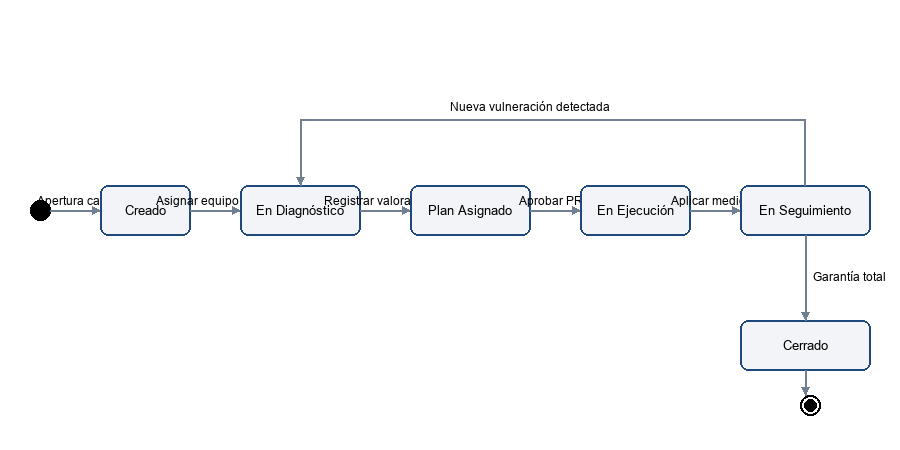
\includegraphics[width=0.95\textwidth]{images/maquina_estados_expediente}
		\caption{Máquina de estados para el Expediente Único de NNA en Taimotla.}
		\label{fig:estadosExpediente}
	\end{center}
\end{figure}

A continuación se describen cada uno de los estados identificados para el expediente:

\begin{description}
	\item[Creado:] El expediente ha sido abierto y el NNA ha sido registrado con sus datos de identidad básicos. Está pendiente la asignación del equipo responsable y la carga de los documentos legales de identidad.
	\item[En Diagnóstico:] El expediente cuenta con un equipo asignado y el acta de nacimiento ha sido validada. Los especialistas se encuentran aplicando las valoraciones clínica, psicológica, jurídica y sociofamiliar.
	\item[Plan Asignado:] Se ha redactado y estructurado el Plan de Restitución de Derechos (PRD) con las medidas aplicables. El PRD está pre-autorizado por el Coordinador en espera de firma por la Dirección.
	\item[En Ejecución:] El Director de la Fundación ha aprobado formalmente el PRD. Las medidas de protección especial y urgentes están siendo ejecutadas y coordinadas con dependencias externas.
	\item[En Seguimiento:] Las medidas de restitución han concluido y el equipo realiza un monitoreo constante del menor para garantizar que no exista riesgo de nueva vulneración de derechos.
	\item[Cerrado:] El caso ha concluido exitosamente tras verificar la restitución duradera e integral de todos los derechos vulnerados del menor.
\end{description}
